\documentclass{standalone}
\usepackage{tikz}
\usetikzlibrary{patterns, positioning}
\usepackage[sfdefault]{ClearSans} %% option 'sfdefault' activates Clear Sans as the default text font
\usepackage[T1]{fontenc}

\begin{document}
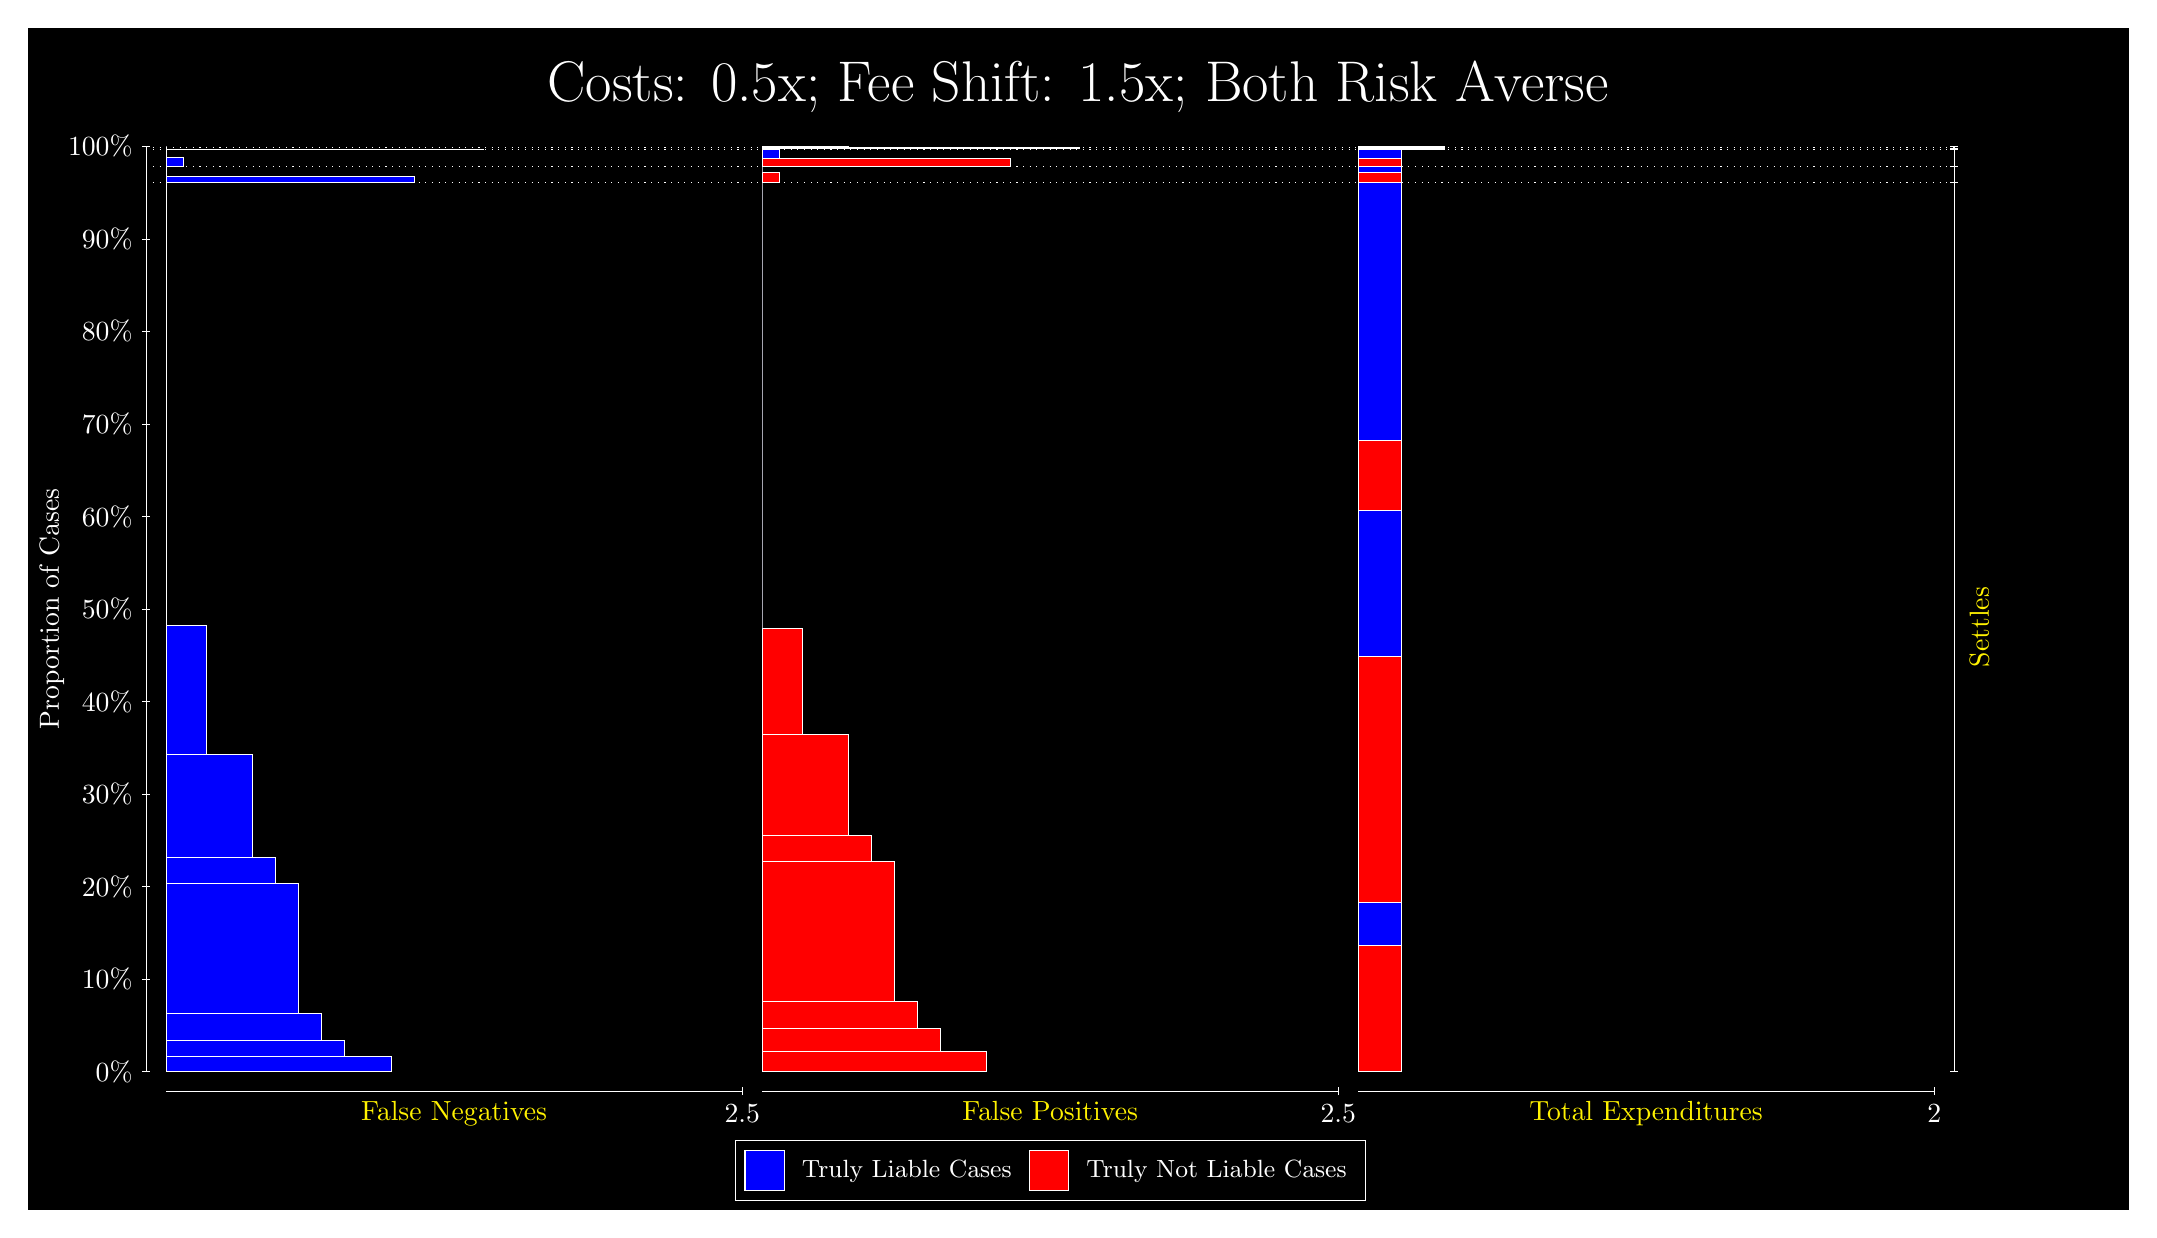
\begin{tikzpicture}
\draw[fill=black] (0,0) rectangle (26.667,15);
\draw[text=white] (0,13.5) rectangle (26.667,15) node[midway] {\huge Costs: 0.5x; Fee Shift: 1.5x; Both Risk Averse};
\draw[white, very thin] (1.5,1.75) -- (1.5,13.5);
\node[rotate=90, text=white, anchor=center] at (0.3, 7.625) {Proportion of Cases};
\draw[white, very thin] (1.45,1.75) -- (1.55,1.75);
\node[text=white, anchor=east] at (1.45, 1.75) {0\%};
\draw[white, very thin] (1.45,2.925) -- (1.55,2.925);
\node[text=white, anchor=east] at (1.45, 2.925) {10\%};
\draw[white, very thin] (1.45,4.1) -- (1.55,4.1);
\node[text=white, anchor=east] at (1.45, 4.1) {20\%};
\draw[white, very thin] (1.45,5.275) -- (1.55,5.275);
\node[text=white, anchor=east] at (1.45, 5.275) {30\%};
\draw[white, very thin] (1.45,6.45) -- (1.55,6.45);
\node[text=white, anchor=east] at (1.45, 6.45) {40\%};
\draw[white, very thin] (1.45,7.625) -- (1.55,7.625);
\node[text=white, anchor=east] at (1.45, 7.625) {50\%};
\draw[white, very thin] (1.45,8.8) -- (1.55,8.8);
\node[text=white, anchor=east] at (1.45, 8.8) {60\%};
\draw[white, very thin] (1.45,9.975) -- (1.55,9.975);
\node[text=white, anchor=east] at (1.45, 9.975) {70\%};
\draw[white, very thin] (1.45,11.15) -- (1.55,11.15);
\node[text=white, anchor=east] at (1.45, 11.15) {80\%};
\draw[white, very thin] (1.45,12.325) -- (1.55,12.325);
\node[text=white, anchor=east] at (1.45, 12.325) {90\%};
\draw[white, very thin] (1.45,13.5) -- (1.55,13.5);
\node[text=white, anchor=east] at (1.45, 13.5) {100\%};

\draw[white, very thin] (24.457,1.75) -- (24.457,13.5);
\draw[white, very thin] (24.407,1.75) -- (24.507,1.75);
\node[anchor=west] at (24.407, 1.75) {};
\draw[white, very thin] (24.407,13.039) -- (24.507,13.039);
\node[anchor=west] at (24.407, 13.039) {};
\draw[white, very thin] (24.407,13.249) -- (24.507,13.249);
\node[anchor=west] at (24.407, 13.249) {};
\draw[white, very thin] (24.407,13.458) -- (24.507,13.458);
\node[anchor=west] at (24.407, 13.458) {};
\draw[white, very thin] (24.407,13.481) -- (24.507,13.481);
\node[anchor=west] at (24.407, 13.481) {};
\draw[white, very thin] (24.407,13.5) -- (24.507,13.5);
\node[anchor=west] at (24.407, 13.5) {};

\draw[white, very thin, fill=blue] (1.75,1.75) rectangle (4.6044,1.9444);
\draw[white, very thin, fill=blue] (1.75,1.9444) rectangle (4.0188,2.1518);
\draw[white, very thin, fill=blue] (1.75,2.1518) rectangle (3.7261,2.4916);
\draw[white, very thin, fill=blue] (1.75,2.4916) rectangle (3.4333,4.1415);
\draw[white, very thin, fill=blue] (1.75,4.1415) rectangle (3.1406,4.471);
\draw[white, very thin, fill=blue] (1.75,4.471) rectangle (2.8478,5.778);
\draw[white, very thin, fill=blue] (1.75,5.778) rectangle (2.2623,7.4127);
\draw[white, very thin, fill=red] (1.75,7.4127) rectangle (1.75,13.039);
\draw[white, very thin, fill=blue] (1.75,13.039) rectangle (4.8971,13.118);
\draw[white, very thin, fill=red] (1.75,13.118) rectangle (1.75,13.249);
\draw[white, very thin, fill=blue] (1.75,13.249) rectangle (1.9696,13.364);
\draw[white, very thin, fill=red] (1.75,13.364) rectangle (1.75,13.458);
\draw[white, very thin, fill=blue] (1.75,13.458) rectangle (5.7754,13.465);
\draw[white, very thin, fill=red] (1.75,13.465) rectangle (1.75,13.481);
\draw[white, very thin, fill=red] (1.75,13.481) rectangle (1.75,13.488);
\draw[white, very thin, fill=blue] (1.75,13.488) rectangle (1.75,13.5);
\draw[white, very thin, fill=red] (9.3189,1.75) rectangle (12.173,2.0059);
\draw[white, very thin, fill=red] (9.3189,2.0059) rectangle (11.588,2.3055);
\draw[white, very thin, fill=red] (9.3189,2.3055) rectangle (11.295,2.6454);
\draw[white, very thin, fill=red] (9.3189,2.6454) rectangle (11.002,4.4257);
\draw[white, very thin, fill=red] (9.3189,4.4257) rectangle (10.709,4.7552);
\draw[white, very thin, fill=red] (9.3189,4.7552) rectangle (10.417,6.0339);
\draw[white, very thin, fill=red] (9.3189,6.0339) rectangle (9.8312,7.3759);
\draw[white, very thin, fill=blue] (9.3189,7.3759) rectangle (9.3189,13.039);
\draw[white, very thin, fill=red] (9.3189,13.039) rectangle (9.5384,13.17);
\draw[white, very thin, fill=blue] (9.3189,13.17) rectangle (9.3189,13.249);
\draw[white, very thin, fill=red] (9.3189,13.249) rectangle (12.466,13.344);
\draw[white, very thin, fill=blue] (9.3189,13.344) rectangle (9.5384,13.458);
\draw[white, very thin, fill=red] (9.3189,13.458) rectangle (9.3189,13.475);
\draw[white, very thin, fill=blue] (9.3189,13.475) rectangle (9.3189,13.481);
\draw[white, very thin, fill=red] (9.3189,13.481) rectangle (13.344,13.488);
\draw[white, very thin, fill=blue] (9.3189,13.488) rectangle (10.417,13.5);
\draw[white, very thin, fill=red] (16.888,1.75) rectangle (17.437,3.3582);
\draw[white, very thin, fill=blue] (16.888,3.3582) rectangle (17.437,3.9054);
\draw[white, very thin, fill=red] (16.888,3.9054) rectangle (17.437,7.0278);
\draw[white, very thin, fill=blue] (16.888,7.0278) rectangle (17.437,8.8721);
\draw[white, very thin, fill=red] (16.888,8.8721) rectangle (17.437,9.7675);
\draw[white, very thin, fill=blue] (16.888,9.7675) rectangle (17.437,13.039);
\draw[white, very thin, fill=red] (16.888,13.039) rectangle (17.437,13.17);
\draw[white, very thin, fill=blue] (16.888,13.17) rectangle (17.437,13.249);
\draw[white, very thin, fill=red] (16.888,13.249) rectangle (17.437,13.344);
\draw[white, very thin, fill=blue] (16.888,13.344) rectangle (17.437,13.458);
\draw[white, very thin, fill=red] (16.888,13.458) rectangle (17.986,13.475);
\draw[white, very thin, fill=blue] (16.888,13.475) rectangle (17.986,13.481);
\draw[white, very thin, fill=red] (16.888,13.481) rectangle (17.986,13.488);
\draw[white, very thin, fill=blue] (16.888,13.488) rectangle (17.986,13.5);
\draw[white, dotted] (1.5,13.039) -- (24.457,13.039);
\draw[white, dotted] (1.5,13.249) -- (24.457,13.249);
\draw[white, dotted] (1.5,13.458) -- (24.457,13.458);
\draw[white, dotted] (1.5,13.481) -- (24.457,13.481);
\draw[white, very thin] (1.75,1.5) -- (9.0689,1.5);
\node[text=yellow, anchor=north] at (5.4094, 1.5) {False Negatives};
\draw[white, very thin] (9.0689,1.45) -- (9.0689,1.55);
\node[text=white, anchor=north] at (9.0689, 1.45) {2.5};

\draw[white, very thin] (9.3189,1.5) -- (16.638,1.5);
\node[text=yellow, anchor=north] at (12.978, 1.5) {False Positives};
\draw[white, very thin] (16.638,1.45) -- (16.638,1.55);
\node[text=white, anchor=north] at (16.638, 1.45) {2.5};

\draw[white, very thin] (16.888,1.5) -- (24.207,1.5);
\node[text=yellow, anchor=north] at (20.547, 1.5) {Total Expenditures};
\draw[white, very thin] (24.207,1.45) -- (24.207,1.55);
\node[text=white, anchor=north] at (24.207, 1.45) {2};

\node[text=yellow, centered, rotate=90] at (24.777, 7.3943) {Settles};





\draw (12.978300999999998,1.5) node[draw=none] (baseCoordinate) {};
\begin{scope}[align=center]
        \matrix[scale=0.5, draw=white, below=0.5cm of baseCoordinate, nodes={draw}, column sep=0.1cm]{
            \node[rectangle, draw, minimum width=0.5cm, minimum height=0.5cm, fill=blue] {}; &
            \node[draw=none, font=\small, text=white] (B) {Truly Liable Cases}; &
            \node[rectangle, draw, minimum width=0.5cm, minimum height=0.5cm, fill=red] {}; &
            \node[draw=none, font=\small, text=white] (B) {Truly Not Liable Cases}; \\
            };
\end{scope}

\end{tikzpicture}
\end{document}